\documentclass[tikz, border=10pt]{standalone}
% Shared preamble — % Shared preamble — % Shared preamble — \input{preamble} in each figure file.
% Compiled via Makefile which sets TEXINPUTS so this file is always found.

% -----------------------------------------------------------------------
% Fonts — matches ntnuthesis.cls
% -----------------------------------------------------------------------
\usepackage[utf8]{inputenc}
\usepackage[T1]{fontenc}
\usepackage[charter, cal=cmcal]{mathdesign} % Charter body + math font
\usepackage[scaled=.88]{berasans}           % Bera sans-serif
\usepackage[scaled=.82]{DejaVuSansMono}     % DejaVu monospace (for \texttt)

% -----------------------------------------------------------------------
% TikZ & PGF
% -----------------------------------------------------------------------
\usepackage{tikz}
\usetikzlibrary{
  positioning,
  arrows.meta,
  fit,
  calc,
  backgrounds,
  shapes.geometric,
  shapes.multipart,
  shapes.symbols,
  shapes.callouts,
  shapes.arrows,
  shapes.misc,
  decorations.pathreplacing,
  decorations.markings,
  matrix,
}
\usepackage{pgf-umlsd}
\usepackage{pgfplots}
\usepackage{pgfplotstable}
\pgfplotsset{compat=1.18}
\usepgfplotslibrary{fillbetween}

% -----------------------------------------------------------------------
% Math
% -----------------------------------------------------------------------
\usepackage{amsmath}

% -----------------------------------------------------------------------
% Color palette
% -----------------------------------------------------------------------
% Semantic NLP / model-diagram colors
\colorlet{tok}{green!35!black}
\colorlet{emb}{yellow!70!orange}
\colorlet{trm}{blue!55!black}
\colorlet{out}{red!70!black}
% General purpose
\colorlet{clrA}{blue!60!black}
\colorlet{clrB}{orange!80!black}
\colorlet{clrC}{green!50!black}
\colorlet{clrD}{red!65!black}
\colorlet{clrE}{violet!70!black}
% Neutral fills
\colorlet{fillLight}{gray!12}
\colorlet{fillMed}{gray!25}

% -----------------------------------------------------------------------
% Global TikZ styles
% NOTE: no blank lines inside \tikzset{} — blank lines produce \par and
%       break pgfkeys parsing.
% -----------------------------------------------------------------------
\tikzset{
  >=Latex,
  % --- generic boxes ---
  box/.style={rectangle, draw, thick, align=center, inner sep=4pt, minimum height=8mm},
  rbox/.style={box, rounded corners=6pt},
  dbox/.style={box, dashed},
  % --- NLP diagram node types ---
  token/.style={rbox, draw=tok!80, fill=tok!20, minimum width=1.8cm, font=\small},
  embed/.style={box, draw=emb!90, fill=emb!30, minimum width=1.4cm},
  trm/.style={ellipse, draw=trm!90, fill=trm!20, minimum width=1.6cm, minimum height=8mm},
  output/.style={rbox, draw=out!90, fill=out!20, minimum width=1.7cm, font=\small},
  % --- arrows ---
  arrow/.style={-{Stealth[length=2mm]}, thick},
  connect/.style={->, thick, gray!65},
  darrow/.style={<->, thick},
  % --- annotation ---
  labelbox/.style={draw, thick, inner sep=4pt, rounded corners=3pt, font=\scriptsize\bfseries},
}
 in each figure file.
% Compiled via Makefile which sets TEXINPUTS so this file is always found.

% -----------------------------------------------------------------------
% Fonts — matches ntnuthesis.cls
% -----------------------------------------------------------------------
\usepackage[utf8]{inputenc}
\usepackage[T1]{fontenc}
\usepackage[charter, cal=cmcal]{mathdesign} % Charter body + math font
\usepackage[scaled=.88]{berasans}           % Bera sans-serif
\usepackage[scaled=.82]{DejaVuSansMono}     % DejaVu monospace (for \texttt)

% -----------------------------------------------------------------------
% TikZ & PGF
% -----------------------------------------------------------------------
\usepackage{tikz}
\usetikzlibrary{
  positioning,
  arrows.meta,
  fit,
  calc,
  backgrounds,
  shapes.geometric,
  shapes.multipart,
  shapes.symbols,
  shapes.callouts,
  shapes.arrows,
  shapes.misc,
  decorations.pathreplacing,
  decorations.markings,
  matrix,
}
\usepackage{pgf-umlsd}
\usepackage{pgfplots}
\usepackage{pgfplotstable}
\pgfplotsset{compat=1.18}
\usepgfplotslibrary{fillbetween}

% -----------------------------------------------------------------------
% Math
% -----------------------------------------------------------------------
\usepackage{amsmath}

% -----------------------------------------------------------------------
% Color palette
% -----------------------------------------------------------------------
% Semantic NLP / model-diagram colors
\colorlet{tok}{green!35!black}
\colorlet{emb}{yellow!70!orange}
\colorlet{trm}{blue!55!black}
\colorlet{out}{red!70!black}
% General purpose
\colorlet{clrA}{blue!60!black}
\colorlet{clrB}{orange!80!black}
\colorlet{clrC}{green!50!black}
\colorlet{clrD}{red!65!black}
\colorlet{clrE}{violet!70!black}
% Neutral fills
\colorlet{fillLight}{gray!12}
\colorlet{fillMed}{gray!25}

% -----------------------------------------------------------------------
% Global TikZ styles
% NOTE: no blank lines inside \tikzset{} — blank lines produce \par and
%       break pgfkeys parsing.
% -----------------------------------------------------------------------
\tikzset{
  >=Latex,
  % --- generic boxes ---
  box/.style={rectangle, draw, thick, align=center, inner sep=4pt, minimum height=8mm},
  rbox/.style={box, rounded corners=6pt},
  dbox/.style={box, dashed},
  % --- NLP diagram node types ---
  token/.style={rbox, draw=tok!80, fill=tok!20, minimum width=1.8cm, font=\small},
  embed/.style={box, draw=emb!90, fill=emb!30, minimum width=1.4cm},
  trm/.style={ellipse, draw=trm!90, fill=trm!20, minimum width=1.6cm, minimum height=8mm},
  output/.style={rbox, draw=out!90, fill=out!20, minimum width=1.7cm, font=\small},
  % --- arrows ---
  arrow/.style={-{Stealth[length=2mm]}, thick},
  connect/.style={->, thick, gray!65},
  darrow/.style={<->, thick},
  % --- annotation ---
  labelbox/.style={draw, thick, inner sep=4pt, rounded corners=3pt, font=\scriptsize\bfseries},
}
 in each figure file.
% Compiled via Makefile which sets TEXINPUTS so this file is always found.

% -----------------------------------------------------------------------
% Fonts — matches ntnuthesis.cls
% -----------------------------------------------------------------------
\usepackage[utf8]{inputenc}
\usepackage[T1]{fontenc}
\usepackage[charter, cal=cmcal]{mathdesign} % Charter body + math font
\usepackage[scaled=.88]{berasans}           % Bera sans-serif
\usepackage[scaled=.82]{DejaVuSansMono}     % DejaVu monospace (for \texttt)

% -----------------------------------------------------------------------
% TikZ & PGF
% -----------------------------------------------------------------------
\usepackage{tikz}
\usetikzlibrary{
  positioning,
  arrows.meta,
  fit,
  calc,
  backgrounds,
  shapes.geometric,
  shapes.multipart,
  shapes.symbols,
  shapes.callouts,
  shapes.arrows,
  shapes.misc,
  decorations.pathreplacing,
  decorations.markings,
  matrix,
}
\usepackage{pgf-umlsd}
\usepackage{pgfplots}
\usepackage{pgfplotstable}
\pgfplotsset{compat=1.18}
\usepgfplotslibrary{fillbetween}

% -----------------------------------------------------------------------
% Math
% -----------------------------------------------------------------------
\usepackage{amsmath}

% -----------------------------------------------------------------------
% Color palette
% -----------------------------------------------------------------------
% Semantic NLP / model-diagram colors
\colorlet{tok}{green!35!black}
\colorlet{emb}{yellow!70!orange}
\colorlet{trm}{blue!55!black}
\colorlet{out}{red!70!black}
% General purpose
\colorlet{clrA}{blue!60!black}
\colorlet{clrB}{orange!80!black}
\colorlet{clrC}{green!50!black}
\colorlet{clrD}{red!65!black}
\colorlet{clrE}{violet!70!black}
% Neutral fills
\colorlet{fillLight}{gray!12}
\colorlet{fillMed}{gray!25}

% -----------------------------------------------------------------------
% Global TikZ styles
% NOTE: no blank lines inside \tikzset{} — blank lines produce \par and
%       break pgfkeys parsing.
% -----------------------------------------------------------------------
\tikzset{
  >=Latex,
  % --- generic boxes ---
  box/.style={rectangle, draw, thick, align=center, inner sep=4pt, minimum height=8mm},
  rbox/.style={box, rounded corners=6pt},
  dbox/.style={box, dashed},
  % --- NLP diagram node types ---
  token/.style={rbox, draw=tok!80, fill=tok!20, minimum width=1.8cm, font=\small},
  embed/.style={box, draw=emb!90, fill=emb!30, minimum width=1.4cm},
  trm/.style={ellipse, draw=trm!90, fill=trm!20, minimum width=1.6cm, minimum height=8mm},
  output/.style={rbox, draw=out!90, fill=out!20, minimum width=1.7cm, font=\small},
  % --- arrows ---
  arrow/.style={-{Stealth[length=2mm]}, thick},
  connect/.style={->, thick, gray!65},
  darrow/.style={<->, thick},
  % --- annotation ---
  labelbox/.style={draw, thick, inner sep=4pt, rounded corners=3pt, font=\scriptsize\bfseries},
}


\begin{document}
    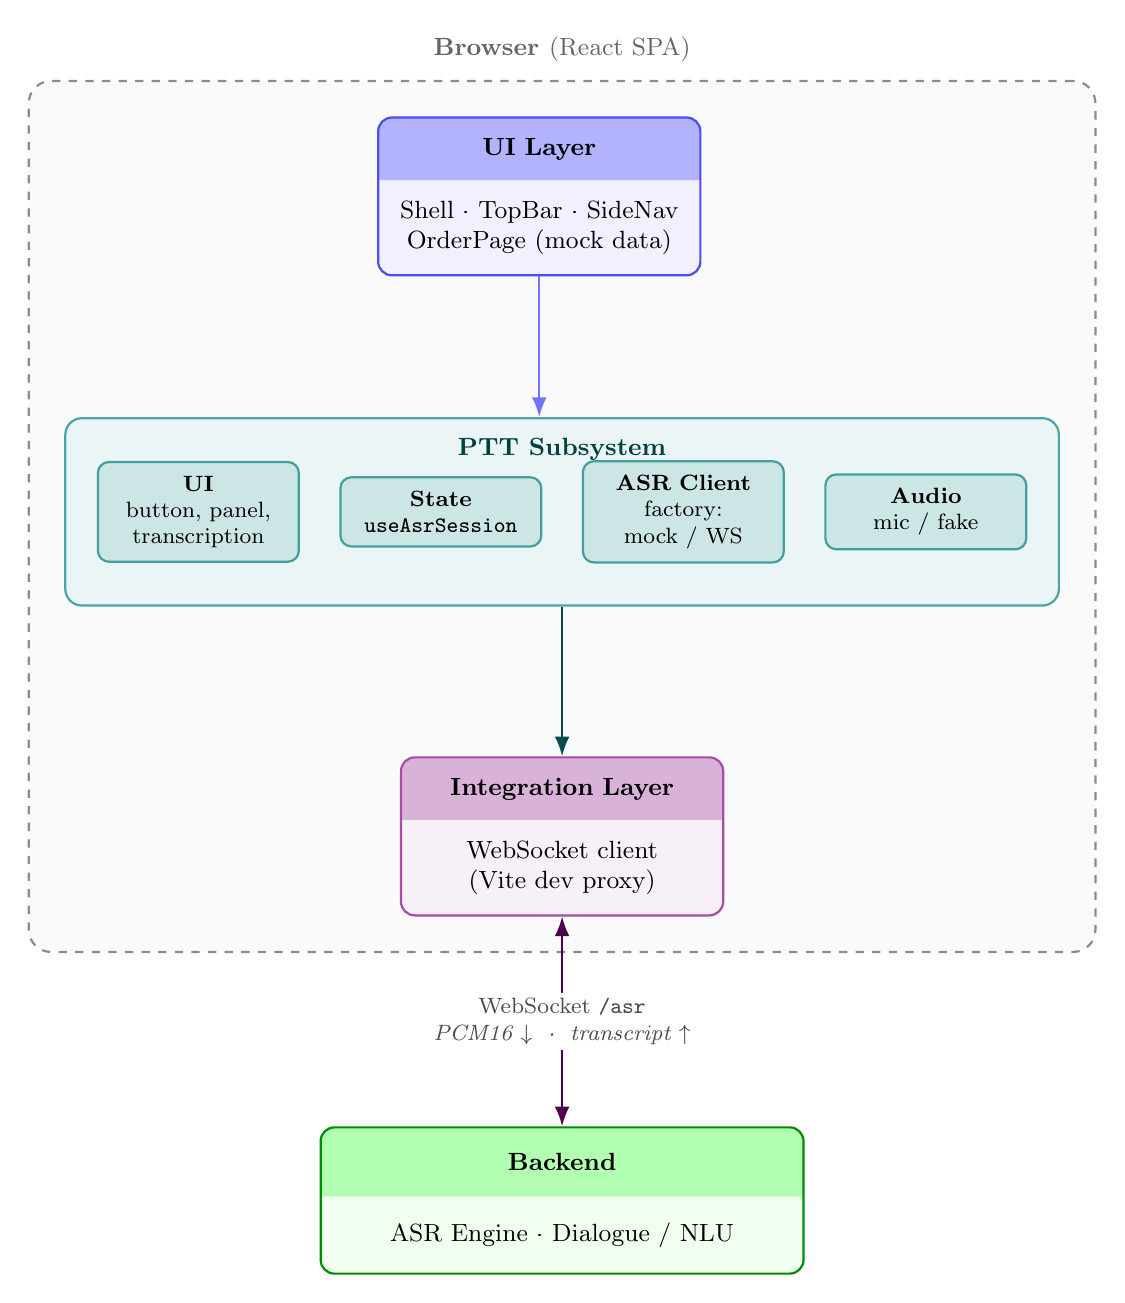
\begin{tikzpicture}[
        font=\small,
        flow/.style     = {-{Latex[length=2.5mm]}, thick, #1},
        flow/.default   = black!70,
        biflow/.style   = {{Latex[length=2.5mm]}-{Latex[length=2.5mm]}, thick, #1},
        biflow/.default = black!70,
        edgelabel/.style = {font=\footnotesize, text=black!70,
                            fill=white, inner sep=2pt, rounded corners=2pt},
        ui/.style={
            draw=blue!70, thick, rounded corners=5pt,
            rectangle split, rectangle split parts=2,
            rectangle split part fill={blue!30, blue!6},
            rectangle split draw splits=false,
            inner sep=7pt, align=center, text width=3.6cm, font=\small,
        },
        module/.style={
            draw=teal!75, thick, rounded corners=4pt,
            fill=teal!20, align=center, inner sep=5pt,
            text width=2.2cm, font=\footnotesize,
        },
        intg/.style={
            draw=violet!70, thick, rounded corners=5pt,
            rectangle split, rectangle split parts=2,
            rectangle split part fill={violet!30, violet!6},
            rectangle split draw splits=false,
            inner sep=7pt, align=center, text width=3.6cm, font=\small,
        },
        backend/.style={
            draw=green!55!black, thick, rounded corners=5pt,
            align=center, inner sep=9pt,
            text width=5.5cm, font=\small,
            rectangle split, rectangle split parts=2,
            rectangle split part fill={green!30, green!6},
            rectangle split draw splits=false,
        },
        host/.style={
            draw=black!45, dashed, rounded corners=8pt,
            fill=black!2, thick, inner sep=0.45cm,
        },
    ]

    %% ── UI Layer ─────────────────────────────────────────────
    \node[ui] (ui) {
        \textbf{UI Layer}
        \nodepart{two}
        Shell · TopBar · SideNav \\ OrderPage (mock data)
    };

    %% ── Invisible anchors for PTT modules (positioning only) ─
    \node[module, draw=none, fill=none, below=2.8cm of ui, xshift=-1.25cm] (anchor_state) {};
    \node[module, draw=none, fill=none, left=0.5cm of anchor_state] (anchor_pttui) {};
    \node[module, draw=none, fill=none, right=0.5cm of anchor_state] (anchor_asrc) {};
    \node[module, draw=none, fill=none, right=0.5cm of anchor_asrc] (anchor_audio) {};

    %% ── PTT Subsystem boundary (drawn FIRST, modules go on top)
    \node[draw=teal!70, thick, rounded corners=6pt,
          fill=teal!8,
          fit=(anchor_pttui)(anchor_state)(anchor_asrc)(anchor_audio),
          inner xsep=0.4cm, inner ysep=1.0cm,
          label={[font=\small\bfseries, text=teal!50!black,
                  anchor=north, yshift=-4pt]north:PTT Subsystem}]
          (ptt) {};

    %% ── PTT modules (drawn AFTER frame so they sit on top) ──
    \node[module] at (anchor_pttui) (pttui)
        {\textbf{UI} \\ button, panel, \\ transcription};
    \node[module] at (anchor_state) (state)
        {\textbf{State} \\ \texttt{useAsrSession}};
    \node[module] at (anchor_asrc) (asrc)
        {\textbf{ASR Client} \\ factory: \\ mock / WS};
    \node[module] at (anchor_audio) (audio)
        {\textbf{Audio} \\ mic / fake};

    %% ── Integration layer ───────────────────────────────────
    \node[intg, below=1.9cm of ptt] (integration) {
        \textbf{Integration Layer}
        \nodepart{two}
        WebSocket client \\ (Vite dev proxy)
    };

    %% ── Browser (SPA) boundary ──────────────────────────────
    \begin{scope}[on background layer]
        \node[host, fit=(ui)(ptt)(integration),
              label={[font=\small\bfseries, text=black!60,
                      anchor=south, yshift=3pt]north:Browser \normalfont(React SPA)}]
              (spa) {};
    \end{scope}

    %% ── Backend ─────────────────────────────────────────────
    \node[backend, below=2.2cm of spa.south] (backend) {
        \textbf{Backend}
        \nodepart{two}
        ASR Engine · Dialogue / NLU
    };

    %% ── Internal arrows (straight down) ─────────────────────
    \draw[flow=blue!55] (ui.south) -- (ui.south |- ptt.north);
    \draw[flow=teal!60!black] (ptt.south) -- (integration.north);

    %% ── WebSocket connection ────────────────────────────────
    \draw[biflow=violet!60!black]
        (integration.south) --
        node[edgelabel, align=center]
            {WebSocket \texttt{/asr} \\
             \itshape PCM16 $\downarrow$ \;·\; transcript $\uparrow$}
        (backend.north);

    \end{tikzpicture}
\end{document}
